\documentclass[10pt,fleqn]{article} % Default font size and left-justified equations
\usepackage[%
    pdftitle={Energétique},
    pdfauthor={Xavier Pessoles}]{hyperref}

    
\input{style/new_style}
\input{style/macros_SII}
\usepackage{multicol}
\usepackage{siunitx}
%\usepackage{picins}
\fichetrue
%\fichefalse

\proftrue

\proffalse

\tdtrue
%\tdfalse

\courstrue
\coursfalse


\def\classe{\textsf{PT -- PT $\star$}}
\def\xxnumpartie{}%Cycle --}
\def\xxpartie{ }

\def\xxnumchapitre{}%Chapitre -- \vspace{.2cm}}
\def\xxchapitre{\hspace{.12cm} }

\def\discipline{Sciences \\Industrielles de \\ l'Ingénieur}
\def\xxtete{Sciences Industrielles de l'Ingénieur}


  
\def\xxposongletx{2}
\def\xxposonglettext{1.45}
\def\xxposonglety{20}
%\def\xxonglet{Part. 1 -- Ch. 3}
\def\xxonglet{\textsf{PT -- PT $\star$}}%Cycle 05}}

\def\xxactivite{Colle 02}
\def\xxauteur{\textsl{Xavier Pessoles}}


\def\xxtitreexo{Roue avant de GC10 -- V8}
\def\xxsourceexo{\hspace{.2cm} \footnotesize{BTS CPI 2017}}


\def\xxcompetences{%
\vspace{-.5cm}
\footnotesize{
\textsl{%
\textbf{Savoirs et compétences :}\\
\vspace{-.2cm}
%\begin{itemize}[label=\ding{112},font=\color{ocre}] 
%\item Mod2.C18.SF1 : Déterminer l’énergie cinétique d’un solide, ou d’un ensemble de solides, dans son mouvement par rapport à un autre solide.
%\item Res1.C1.SF1 : Proposer une démarche permettant la détermination de la loi de mouvement.
%\item Mod1.C5.SF2 : Déterminer la puissance des actions mécaniques extérieures à un solide ou à un ensemble de solides, dans son mouvement rapport à un autre solide.
%\item Mod1.C5.SF3 : Déterminer la puissance des actions mécaniques intérieures à un ensemble de solides.
%\end{itemize}
}}}

\def\xxfigures{
\includegraphics[width=.75\textwidth]{images/fig_00}
}%figues de la page de garde


\def\xxpied{%
%Cycle 05 -- Modélisation mécanique -- Énergétique\\% afin de valider leurs performances.\\
%Chapitre 1 -- \xxactivite%
}

\setcounter{secnumdepth}{5}
%---------------------------------------------------------------------------


\begin{document}
%\chapterimage{png/Fond_Cin}
\input{style/new_pagegarde}
\vspace{4cm}
\pagestyle{fancy}
\thispagestyle{plain}


\def\columnseprulecolor{\color{ocre}}
\setlength{\columnseprule}{0.4pt} 

%\ifprof
%\else
%\begin{multicols}{2}
%\fi
\section*{Mise en situation}
\ifprof
\else
\fi

On s'intéresse à la roue avant et au pivot de roue d'une voiture de course et plus particulièrement au moyeu de roue.

\begin{center}
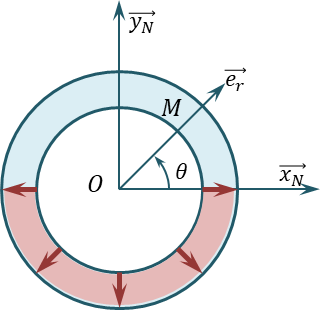
\includegraphics[height=8.5cm]{images/fig_02}
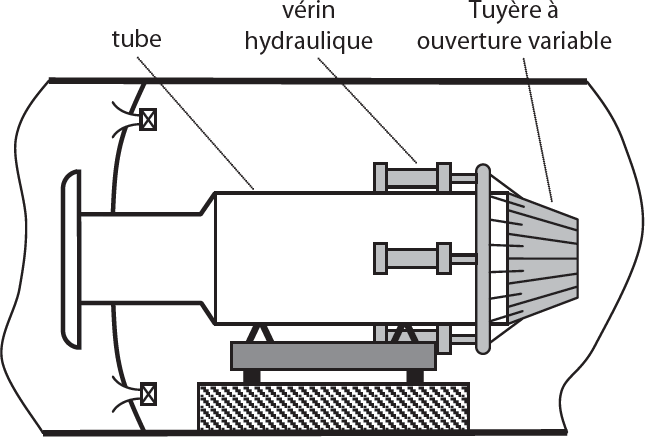
\includegraphics[height=8.5cm]{images/fig_03}
\end{center}

Le plan d'ensemble au verso montre l'assemblage du moyeu avec les autres constituants. 

\subsection*{Analyse des spécifications géométriques et dimensionnelles}

\begin{minipage}[c]{.6\linewidth}
\subparagraph{}
\textit{Expliquer quelle(s) fonction(s) du produit justifie l'existence des spécifications suivantes :
\includegraphics[width=2cm]{images/gps_01} et \includegraphics[width=2cm]{images/gps_02}.}


\subparagraph{}
\textit{Décrire les spécifications suivantes :
\includegraphics[height=.6cm]{images/gps_01}, \includegraphics[height=.6cm]{images/gps_02}, \includegraphics[height=.6cm]{images/gps_03}, \includegraphics[height=.6cm]{images/gps_04} et \includegraphics[height=.7cm]{images/gps_05}.}

\subparagraph{}
\textit{Quelle serait la conséquence d'un ajout du modificateur du maximum de matière sur l'intervalle de tolérance de la spécification de coaxialité ? sur l'élément de référence ?}

\end{minipage} \hfill
\begin{minipage}[c]{.38\linewidth}

\begin{center}
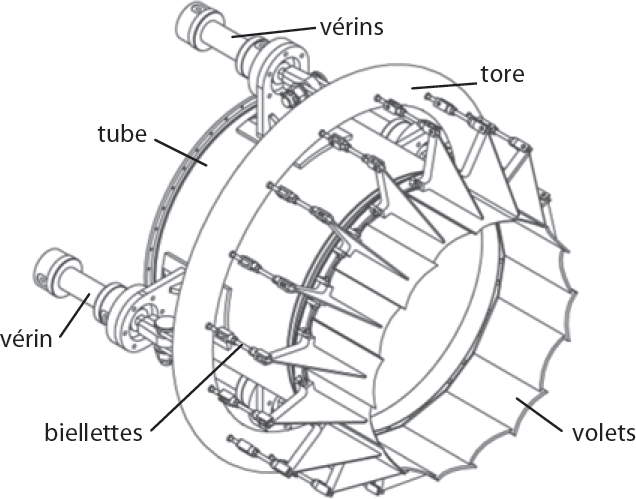
\includegraphics[width=.9\linewidth]{images/fig_04}
\end{center}
\end{minipage}
\subsection*{Analyse des procédés de fabrication}
\subparagraph{}
\textit{Donner l'ensemble des moyens de fabrications ayant mené à la réalisation du moyeu de roue.}

\subparagraph{}
\textit{Proposer une gamme de fabrication permettant de réaliser le moyeu.}

%\end{multicols}




\begin{center}
\rotatebox{270}{\includegraphics[height=\linewidth]{images/plan_01}}
\rotatebox{270}{\includegraphics[height=\linewidth]{images/plan}}

%{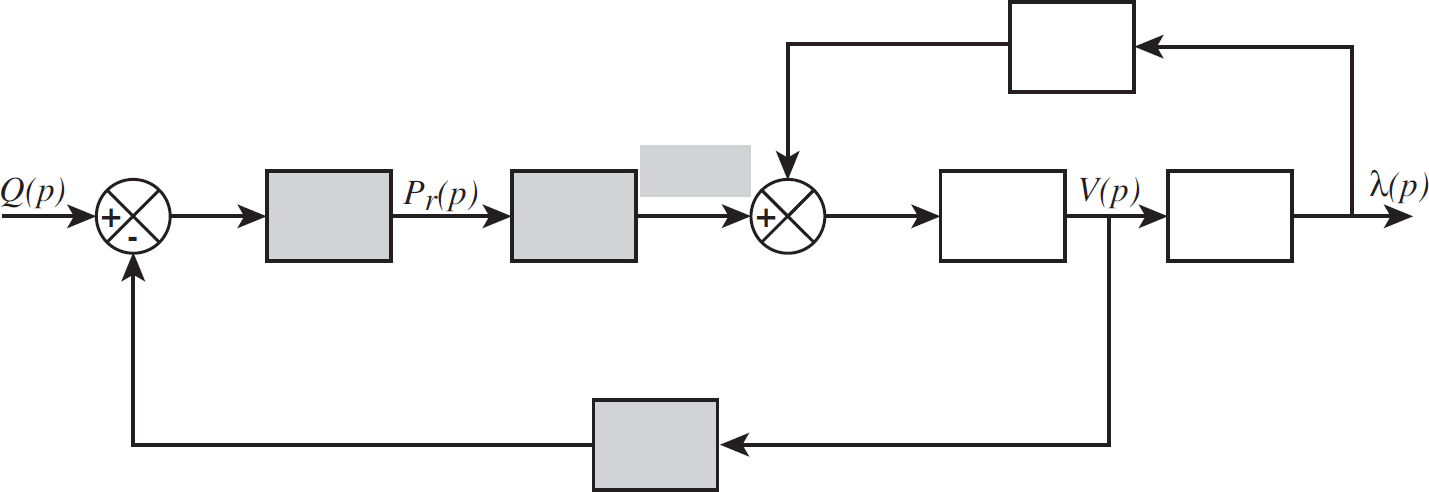
\includegraphics[width=\linewidth]{images/fig_06}}
\end{center}


\end{document}

\subparagraph{}\textit{}
\ifprof
\begin{corrige}~\\
\end{corrige}
\else
\fi




\subparagraph{}\textit{}
\ifprof
\begin{corrige}~\\
\end{corrige}
\else
\fi

\subparagraph{}\textit{}
\ifprof
\begin{corrige}~\\
\end{corrige}
\else
\fi

\subparagraph{}\textit{}
\ifprof
\begin{corrige}~\\
\end{corrige}
\else
\fi

\subparagraph{}\textit{}
\ifprof
\begin{corrige}~\\
\end{corrige}
\else
\fi

\subparagraph{}\textit{}
\ifprof
\begin{corrige}~\\
\end{corrige}
\else
\fi

\subparagraph{}\textit{}
\ifprof
\begin{corrige}~\\
\end{corrige}
\else
\fi
\begin{center}
%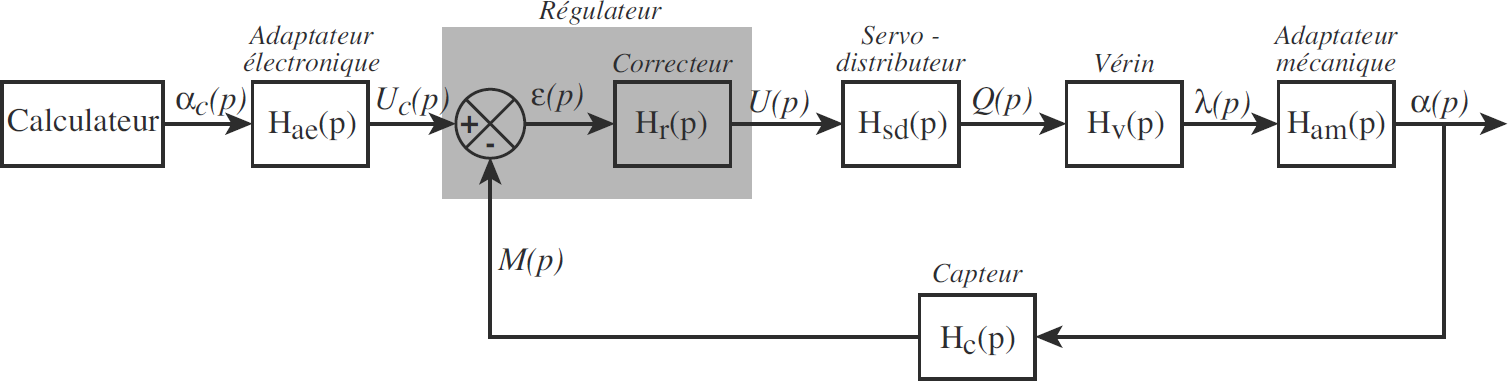
\includegraphics[width=\linewidth]{images/fig_05}
\end{center}
